% Chapter Template

\chapter{Fabrication and Characterization of Polymeric Fibers through Near-Field Electrospinning} % Main chapter title

\label{Chapter:4}

The fabrication and characterization of polymeric fibers is addressed in this chapter as the last screening procedure to select the PEO/SU-8 replacement. The PEO/SU-8 replacement is to produce microscopic polymer fibers with potential for the fabrication of carbon nano-wires. This chapter reports PEO, PS, PSB, and PVK micro-fibers fabricated by low-voltage near-field electrospinning. The fabrication process is carried on to study the influence of applied voltage on the fiber diameter. The materials and sample preparation for the LV-NFES process are the same as those used in the rheological analyses in Chapter \ref{Chapter:3}.

\section{Near-Field Electrospinning Setup}

\begin{figure}[!th]
\centering
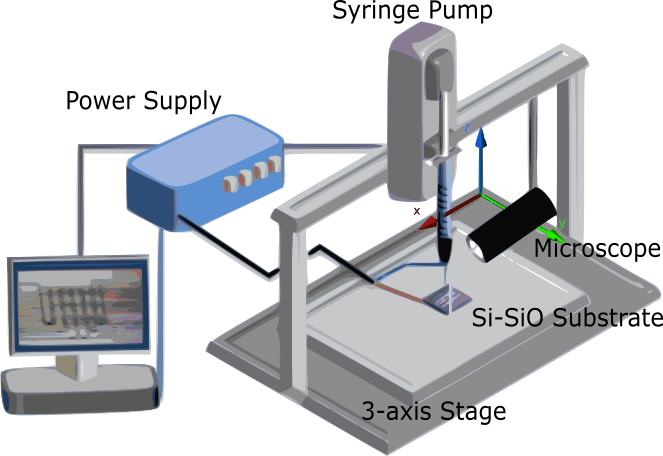
\includegraphics[scale=0.50]{./Figures/NFESsetup.png}
\decoRule
\caption[NFES experimental setup]{NFES experimental setup. Adapted from \cite{Floreshernandez2020}}
\label{fig:NFESsetup}
\end{figure}

The near-field apparatus (Figure \ref{fig:NFESsetup}) is comprised by a high voltage supply (HVS448 3000 V, LabSmith, Livermore, CA, USA), a three-axis stage, syringe pump (Pump 11 Elite, Harvard Apparatus, Cambridge, MA, USA). Samples were prepared as per the rheology measurements in Chapter \ref{Chapter:3}. Experiments were conducted with 1 milliliter slip-tip insulin syringes with 21 gauge precision tips (Nordson Engineered Fluid Dispensing, Westlake, OH, USA). The power supply and 3-axis stage are controlled through a desktop computer, while the syringe pump is controlled manually. Fiber depositions were placed on a $\textrm{Si}-\textrm{SiO}_2$ wafer. The voltage between the nozzle tip and the collector was varied between $200 [\textrm{V}]$ and $600 [\textrm{V}]$ in increments of $100 [\textrm{V}]$, keeping a constant current of $10 \textrm{ } \mu \textrm{A}$. For applied voltages under $400 [\textrm{V}]$, the electric field was not strong enough to overcome the surface tension of the polymer solution and initiate the jet. To enable the fiber deposition at low voltages, the polymer jet was manually initialized by breaking the surface tension with a sharp glass tip. The working distance $L$ and stage velocity was set at a constant values for all the experiments at $0.5 mm$ and $10 mm/s$ respectively. The syringe pump was set at a steady flow rate of $0.04 \mu \textrm{L} / \textrm{min}$.

\begin{figure}[!th]
\centering
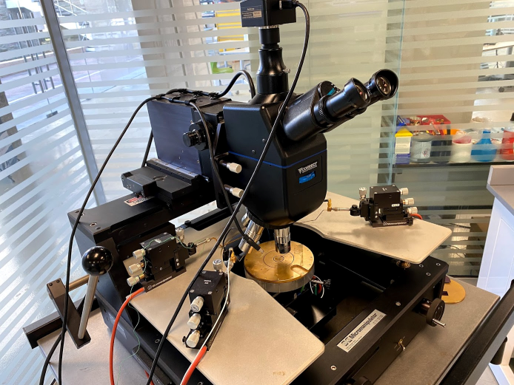
\includegraphics[scale=0.50]{./Figures/microscope.png}
\decoRule
\caption{Correct, Seiwa Optical - Optical Microscope}
\label{fig:microscope}
\end{figure}

The applied voltage range was set in a range between $200 [\textrm{V}]$ and $600 [\textrm{V}]$, since within that range fibers were able to electrospun into continuous and straight fibers. As shown in Figure \ref{fig:lowVoltageHighVoltage}, PEO/SU-8 fibers are produced with a meander morphology when the applied voltage is around $900 [\textrm{V}]$. Under $600 [\textrm{V}]$, straight and aligned fibers were fabricated and characterized.

The calculated critical concentrations in Chapter \ref{Chapter:3} (Table \ref{tab:calculatedSpinnableConcentrations}) are used for the fabrication of polymeric fibers. One set of experiments was conducted for each polymer-solvent system to study the effect of applied voltage on fiber diameter. The morphology of the fibers was characterized with an optical microscope (Correct, Seiwa Optical, Dallas, TX, USA, Figure \ref{fig:microscope}). Each sample was measured at 30+ points within the microscope field of view (Appendix \ref{Appendix_MicroscopyChar}).

\begin{figure}[!th]
\centering
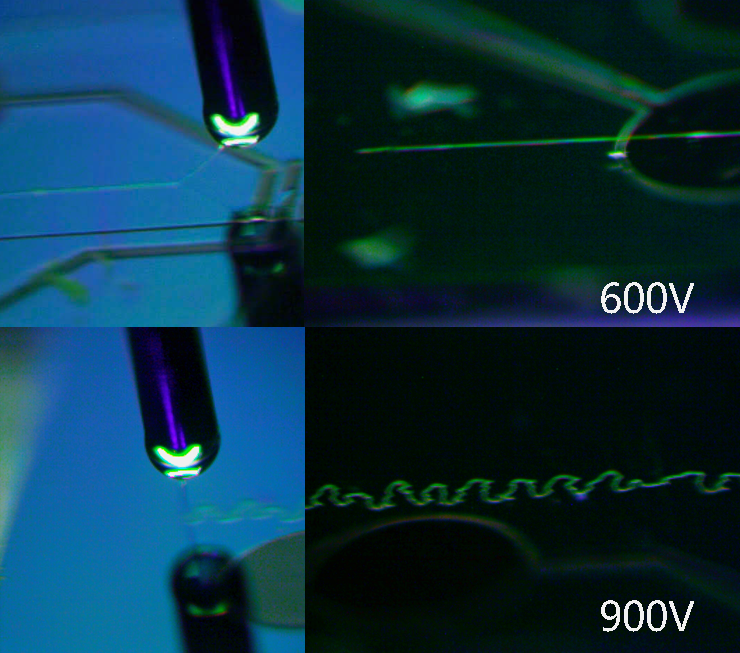
\includegraphics[scale=0.40]{./Figures/lowVoltageHighVoltage.png}
\decoRule
\caption{Effect of applied voltage in fiber morphology}
\label{fig:lowVoltageHighVoltage}
\end{figure}

\section{Results}

\begin{figure}[!th]
\centering
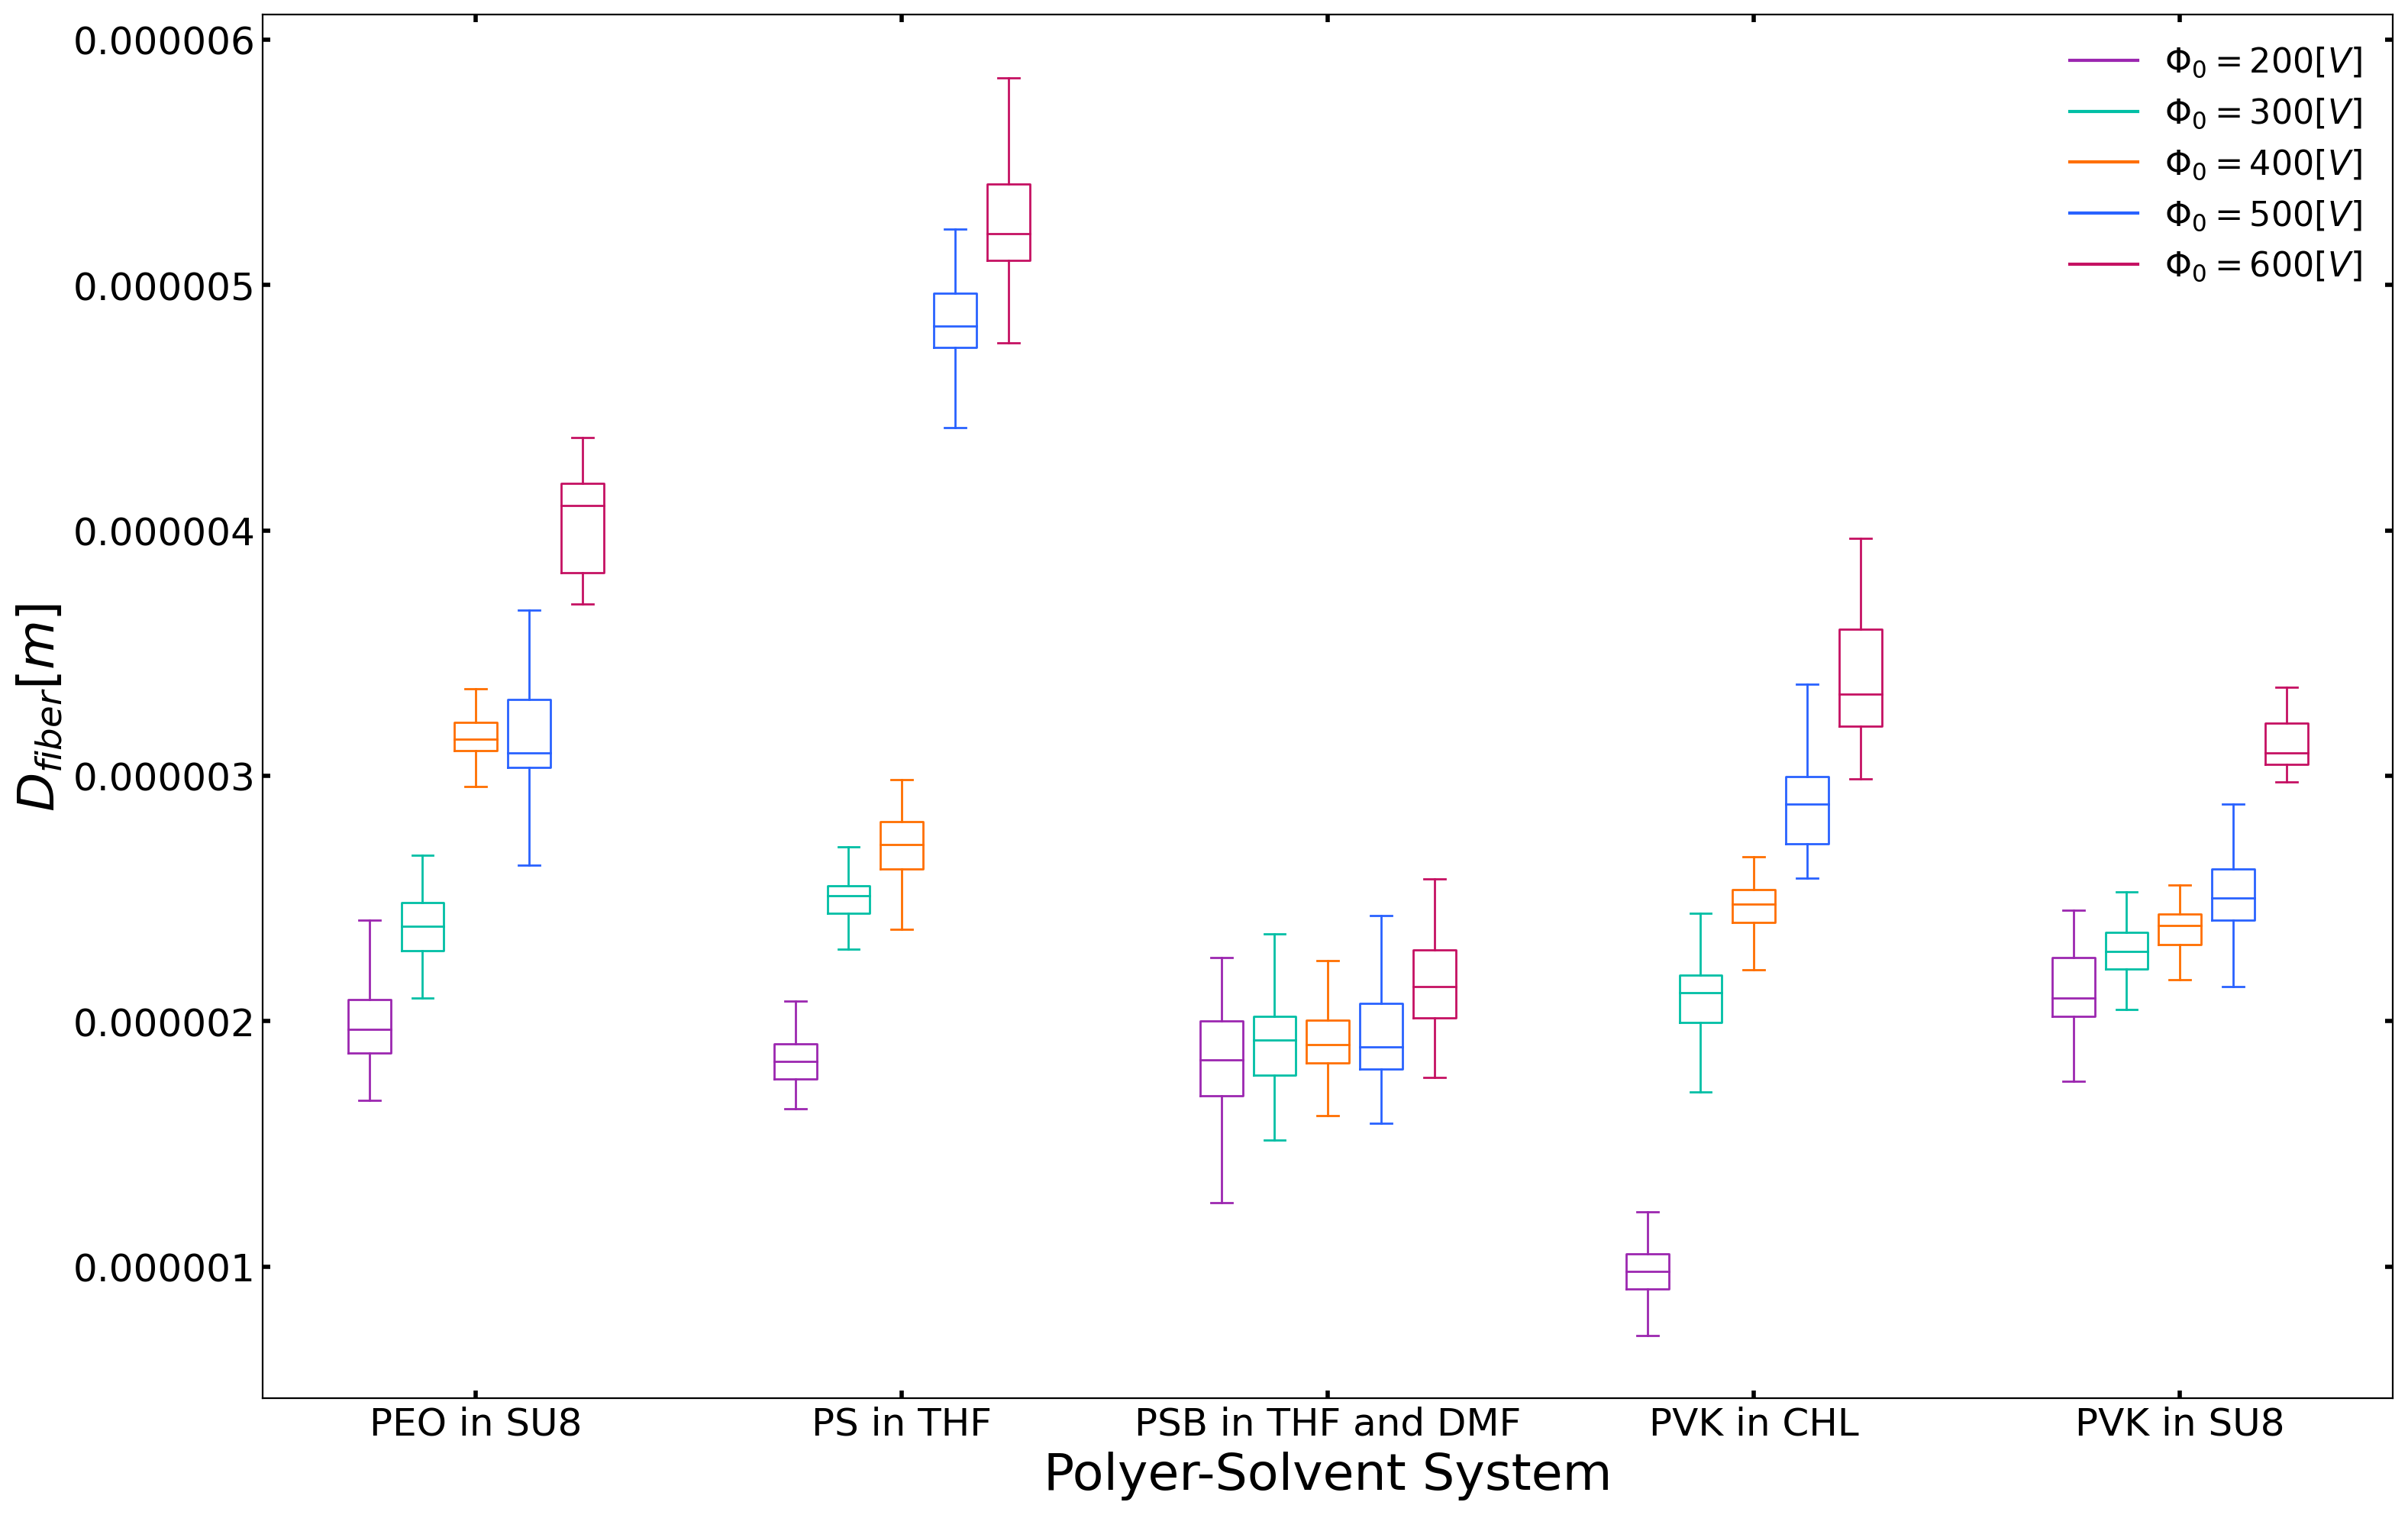
\includegraphics[width=\textwidth]{./Figures/boxplotsFiberDiameter.png}
\decoRule
\caption[Diameter of fibres for all the experiments]{Diameter of fibres for all the experiments with varing applied voltage $\Phi_0$. Appendix \ref{Appendix_FiberDiameters}}
\label{fig:boxplotsFiberDiameter}
\end{figure}

Figure \ref{fig:boxplotsFiberDiameter} shows a dependence of fiber diameter as a function of the applied voltage and confirms what was already noticed in the correlation matrix and the adimensional analysis in Chapter \ref{Chapter:2}, as lower voltages yield fibers with thinner diameters. This results verify the electro-spinnability of oxygen-less polymers by NFES into fibers of $1 \mu m$ to $5 \mu m$ in diameter. PS presented complications during the NFES process as fibers of this polymer do not adhere onto the substrate making them prone to fracture or substrate abandonment, specially when printing fibers of thin diameters. To ease this complication the working distance $L$ can be reduced to let the fibers dry on the surface and prevent complete solidification while traveling the distance $L$. The increase in applied voltage can also help with this problem as more material is pulled out of the dispensing needle, however this two fixes will translate into thicker fibers.

The effect of applied voltage on fiber diameter can be contributed to the effect of the electric field on the surface tension of the polymer solution drop. Bateni and coworkers \cite{Bateni2005} have shown that surface tension increases with increasing applied voltage. Bateni also states that the effect of an electric field is stronger on alcohols with higher molecular weights \cite{Bateni2005}. Bateni's findings agree with Zhenan Bao's statements regarding polymers with OH functional groups are more easily electrospun than those without functional groups \cite{Liu2015a, Bateni2005}. Since the tested polymers are of different molecular weights, the effect of applied voltage is more significant in the PEO/SU-8 formulation as PEO has the highest molecular weight. On the other hand, the PSB in THF and DMF solution was the least affected by changes in applied voltage as PSB has the smallest molecular weight. Disregarding the molecular weight, the PS formulation has higher variation in fiber diameter. This outcome can be explained by the poor adhesion of the fibers to the substrate, as explained above. The effect of the applied voltage between the two PVK samples present some differences. The PVK in CHL solution has a stronger reaction to the electric field than the PVK in SU-8 formulation. This difference can be attributed to the fact that SU-8 is comprised by a series of monomers of low molecular weight.

The PVK and CHL system was the one that behaved with more similarity as the control sample of SU-8 and PEO. Uniform, $700 \textrm{ nm}$ diameter fibers were achieved with PVK and CHL at the lowest voltage setting ($200 \textrm{ V}$). Given the similarities with the control sample, PVK was choosen to replace the PEO to increase the spinnability of SU8. Therefore, the PVK in SU-8 system was tested in the same conditions as the previous experiments. Both polymers (PEO and PVK) in SU-8 yield parallel results in fiber morphology and in electrospinning preformanc. However, at high voltages, the PVK solution produced thinner fibers than those produced by the PEO solution. Moreover, as PVK does not contain any additional oxygen content in its structure, adding PVK can be a better alternative to electrospun SU-8 based fibers intended for carbonization as thinner fibers will have better opportunities to survive the pyrolysis process without breaking.

On the other hand, the polymer-solvent systems comprised by Poly(Styrene-co-Butadiene) (PSB) in 1-Methyl-2-Pyrrolidinone (NMP) and Poly(Styrene-co-alpha-Methylstyrene) (PSMS) in N,N-Dimethylformamide (DMF) were unable to yield fibers. In the case of the PSB/NMP solutions, a hard shell was formed around the polymer drop at the tip of the nozzle preventing the jet to initiate, which causes clogging. Seems that rapid volatilization of NMP is not the case as PSB was successfully electrospun with more volatile solvents (THF and DMF). Notice that vapor pressure of NMP is around $39 \textrm{Pa}$ at $25^{\circ} C$, THF and DMF have vapor pressures of about $19.3 \textrm{kPa}$ at $20^{\circ} C$ and $0.49 \textrm{kPa}$ at $25^{\circ} C$ respectively. \cite{ICSCs} On the other hand, PSMS in DMF was not able to produce fibers as the jet was not initiated. After noticing that que calculated critical concentration $c^*$ is not spinnable the solutions of 10 and 15 $wt\%$ were also tested in the NFES apparatus with no success. The cause of the non-spinnable nature of PSMS can be laid on the fact that PSMS pellets were brittle and capable of making fine PSMS dust with ease, unlike PS and PSB pellets which have an elastic behavior.
